\documentclass{report}
\usepackage[left=3cm]{geometry}
\usepackage{verbatim}
\usepackage{graphicx}
\usepackage{tabularx}
\setlength{\extrarowheight}{5pt}

\begin{document}
\title{Advacend Object-oriented Programming Project Report}
\author{MINGKUN YANG ID:900506-T008\\
albertnetymk@gmail.com\\
}
\maketitle

\section{Framework}
\begin{figure}[t]
  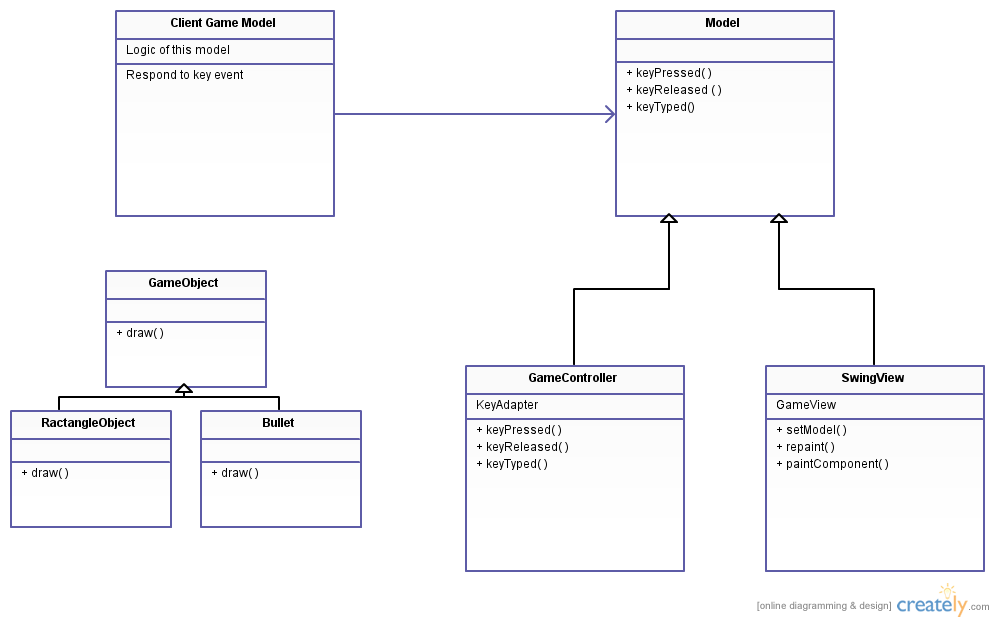
\includegraphics[scale=0.5]{framework.png}
  \caption{MVC game framework}
\end{figure}
The ``GameController'' is the part in this framework has intelligence. It will accept user's input and forward them to client game model, if the key 
event are not the predefined command. In the implementation of ``GameController'', one thread is used to communicate with the model directly.

The ``GameView'' is responsible for painting the playground. In normal cases, client will not need to deal with this class.

The ``GameModel'' is the super class meant to be extended by client game model. This is where the game logic will exist, and application developers 
will deal with key events forwards from ``GameController''. In fact, as for dealing with key events, clients should implement ``keyPressed'', 
``keyReleased'' and ``keyTyped'' methods, just like ``KeyAdapter'' class. In this case, clients have complete control of the key events. In this 
class, there is one method called ``cleanUp'', which is meant to be called, when this game is over. With this, the application can have the freedom 
do some data collection or cleaning up after the game. Another method called ``shutdownView'' will also be called when the game is finished. With 
this method, application developers can present one view to users to show some information.

The ``GameOverException'' is the class, that will be instantiated, and threw.

The ``GameObject'' is the super class for all objects appear in the game view. Only ``draw'' method is define in this class. After implementing this 
method, application developer can do whatever suit their needs.

The ``SwingConsole'' is the class calling the constructor of ``SwingMain''. The look and feel of the application is managed in here. The default look 
and feel is that of this platform this application is running.
\section{Application Development}
The ``SwingMain'' is the frame contains the ``GameView''. If application developers are satisfied with the default configuration, they can just add 
one menu item. However, application developers have freedom change it, for it is not part of this game framework.

With the help of this framework, there are not much to do except implementing the logic of the game. Therefore, application developers only need to 
create new game model, in which the rules of the game are defined. In addition, it might be possible to create several subclasses of ``GameObejct'', 
that will be used in this game.
\section{Patterns}
\begin{itemize}
	\item Observer pattern \\
		This pattern is used for views to reflect the change of the model. Whenever new command comes in, and the state of the game model changes, 
		view will update.
	\item Strategy pattern \\
		A few methods are defined in GameModel, which are meant to be implemented in subclasses. The implementation depends on the particular logic 
		of the game model.
	\item Composition pattern \\
		In the instance of ``GameController'', one thread exists there. This thread is responsible for driving this game and communicate with the 
		model directly.
	\item Factory pattern \\
		The classes implementing ``GameFactory'' will creat new game model based on the same dimension.
\end{itemize}
\section{Changing logs of the framework}
In the original framework, the methods for accepting key event are defined as part of framework, which means that if application developers want to 
have fine control of key events, they have to change this framework. Therefore, in the new framework, key events will be forwarded to the thread, 
then thread will forward the key events to the game model. In the game model, application developers can deal with them.

In the original framework, ``GameThread'' is one public class, but this class is not meant to be used by application developers. Therefore, in the 
new framework, ``GameThread'' is one nested class in ``GameController''. Since ``GameController'' is the only class uses this, it makes sense to put 
it in there. Considering that the controller is the only part, that has intelligence in this MVC architecture, one thread should be in that class.

It is possible that application developers want to save some information after the game is over. Methods called ``cleanUp'', and ``shutdownView'' in 
``GameModel'' are defined, so that application developers can override them, which will be called when the game is over.
\section{Changing logs of the game}
Both of the games are using the new framework.

Originally, several variables and methods are added to ``GameModel'' so that it is possible to keep track of how many points which player has got. 
The current implementation of this is just one simple example to do this. One separate class will be much better in complex system. On the second 
thoughts, it will make more sense to put the information concerning scores in the particular game model, not in the ``GameModel'' super class. 
Otherwise, even some games, that do not use such information will carry this. Therefore, the information concerning scores is add in ``GoldModel'', 
the particular game model.
\end{document}
